%%%%%%%%%%%%%%%%%%%%%%%%%%%%%%%%%%%%%%%%%%%%%%%%%%%%%%%%%%%%%%%%%%%%%%%%%%%%%%
% LIAMA visiting committee - 9 November 2010
%%%%%%%%%%%%%%%%%%%%%%%%%%%%%%%%%%%%%%%%%%%%%%%%%%%%%%%%%%%%%%%%%%%%%%%%%%%%%%

\documentclass{beamer}

\usepackage{beamerthemesplit}
\usepackage{url}
\usepackage{graphicx}

\newcommand\toc{\begin{f}{Outline}\tableofcontents[currentsection]\end{f}}

\newenvironment{f}[1]{\begin{frame}\frametitle{#1}}{\end{frame}}
\renewenvironment{i}{\begin{itemize}}{\end{itemize}}
\newenvironment{e}{\begin{enumerate}}{\end{enumerate}}
\renewenvironment{c}{\begin{center}}{\end{center}}
\renewenvironment{t}[1]{\begin{tabular}{#1}}{\end{tabular}}
\newenvironment{p}{\begin{prooftree}}{\end{prooftree}}

\newcommand\red{\textcolor{red}}
\newcommand\orange{\textcolor{orange}}
\newcommand\violet{\textcolor{violet}}
\newcommand\green{\textcolor{green}}
\newcommand\blue{\textcolor{blue}}

\newcommand\vsp[1][3mm]{\vspace*{#1}}
\newcommand\hsp[1][3mm]{\hspace*{#1}}

\newcommand\A\Rightarrow

%%%%%%%%%%%%%%%%%%%%%%%%%%%%%%%%%%%%%%%%%%%%%%%%%%%%%%%%%%%%%%%%%%%%%%%%%%%%%%

\title{SimSoC certification}
\author{F. Blanqui (INRIA)}
\institute{
\red{FORMES project}\\[5mm]
LIAMA - Tsinghua University\\[5mm]
\red{\url{http://formes.asia/}}}
\date{\tiny 9 November 2010}

\begin{document}

\frame\titlepage

%%%%%%%%%%%%%%%%%%%%%%%%%%%%%%%%%%%%%%%%%%%%%%%%%%%%%%%%%%%%%%%%%%%%%%%%%%%%%%

\begin{f}{Participants}

\begin{i}
\item
Fr\'ed\'eric Blanqui (CR INRIA)
\item
Claude Helmstetter (postdoc INRIA)
\item
Vania Joloboff (DR INRIA)
\item
Jean-Francois Monin (Pr UJF/CNRS)
\item
Xiaomu Shi (PhD student UJF)
\end{i}

\end{f}

%%%%%%%%%%%%%%%%%%%%%%%%%%%%%%%%%%%%%%%%%%%%%%%%%%%%%%%%%%%%%%%%%%%%%%%%%%%%%%

\begin{f}{SimSoC}

\begin{i}\itemsep+3mm
\item
\blue{fast bit-accurate simulator for systems on chips including:}
\begin{i}
\item processors (ARM, PPC, MIPS)
\item memory management unit (MMU)
\item memories (RAM, flash NAND/NOR)
\item communication devices (UART, Ethernet)
\end{i}
\item
\blue{average speed: 88 Mips}
\item
\blue{can simulate operating systems (Linux) and software on top}
\item
\blue{written in C++ using SystemC/TLM ($\sim$60 Kloc)}
\end{i}

\vsp\pause
\red{$\A$ how to make sure that the simulation is correct?}

\end{f}

%%%%%%%%%%%%%%%%%%%%%%%%%%%%%%%%%%%%%%%%%%%%%%%%%%%%%%%%%%%%%%%%%%%%%%%%%%%%%%

\begin{f}{ARM architecture reference manual version 6}

\begin{i}\itemsep+3mm
\item \blue{1138 pages\ldots}
\begin{i}
\item 37 registers + 15 system coprocessor registers
\item 7 processors mode
\item 7 exception processing modes
\item 5 addressing modes
\end{i}
\item \blue{220 instructions described on 600 pages}
\item \blue{for each instruction, it is provided:}
\begin{i}
\item binary encoding
\item assembly syntax
\item pseudo-code describing its semantics
\item explanations, remarks and examples
\end{i}
\end{i}

\vsp\pause
\red{$\A$ automated code generation is safer and faster}

\end{f}

%%%%%%%%%%%%%%%%%%%%%%%%%%%%%%%%%%%%%%%%%%%%%%%%%%%%%%%%%%%%%%%%%%%%%%%%%%%%%%

\begin{f}{Example: ADC instruction encoding (page 154)}

\begin{figure}
% ps
%\vsp[-20mm]\hsp[-5mm]\rotatebox{-90}{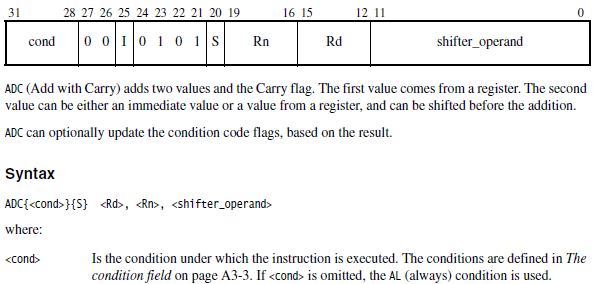
\includegraphics[scale=.6]{adc1}}
% pdf
\vsp[-10mm]\hsp[-9mm]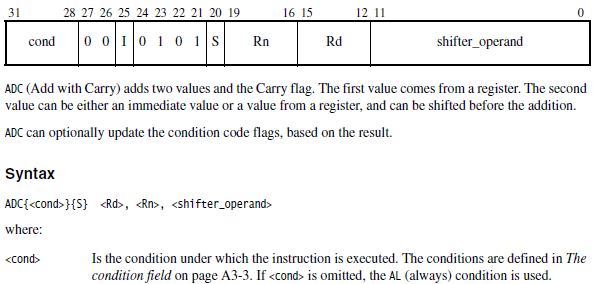
\includegraphics[scale=.6]{adc1}
\end{figure}

\end{f}

%%%%%%%%%%%%%%%%%%%%%%%%%%%%%%%%%%%%%%%%%%%%%%%%%%%%%%%%%%%%%%%%%%%%%%%%%%%%%%

\begin{frame}[fragile]{Example: ADC instruction semantics (page 155)}

\begin{verbatim}
if ConditionPassed(cond) then
  Rd = Rn + shifter_operand + C Flag
  if S == 1 and Rd == R15 then
    if CurrentModeHasSPSR() then
      CPSR = SPSR
    else UNPREDICTABLE
  else if S == 1 then
    N Flag = Rd[31]
    Z Flag = if Rd == 0 then 1 else 0
    C Flag = CarryFrom(Rn + shifter_operand + C Flag)
    V Flag = OverflowFrom(Rn + shifter_operand + C Flag)
\end{verbatim}

\end{frame}

%%%%%%%%%%%%%%%%%%%%%%%%%%%%%%%%%%%%%%%%%%%%%%%%%%%%%%%%%%%%%%%%%%%%%%%%%%%%%%

\begin{f}{Code generation}

\begin{figure}
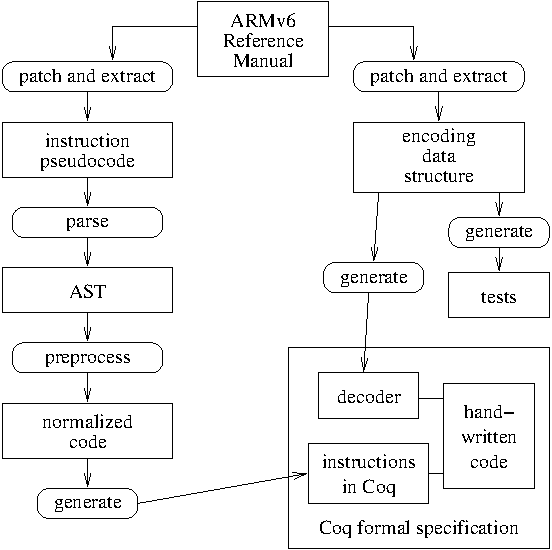
\includegraphics[scale=.8]{generationStep}
\end{figure}

\end{f}

%%%%%%%%%%%%%%%%%%%%%%%%%%%%%%%%%%%%%%%%%%%%%%%%%%%%%%%%%%%%%%%%%%%%%%%%%%%%%%

\begin{frame}[fragile]{Example of generated Coq code}

{\small\begin{verbatim}
Definition ADC_step (s0 : state) (S : bool) (cond : opcode)
  (d : regnum) (n : regnum) (shifter_operand : word) : result :=
  if_then (ConditionPassed s0 cond)
    (block (
      set_reg d (add (add (reg_content s0 n) shifter_operand) ((cpsr s0)[Cbit])) ::
      if_then_else (andb (zeq S 1) (zeq d 15))
        (if_then_else (CurrentModeHasSPSR s0)
          (set_cpsr (spsr s0 None))
          (unpredictable EmptyMessage))
        (if_then (zeq S 1)
          (block (
            set_cpsr_bit Nbit ((reg_content s0 d)[31]) ::
            set_cpsr_bit Zbit (if zeq (reg_content s0 d) 0 then repr 1 else repr 0) ::
            set_cpsr_bit Cbit (CarryFrom_add3 (reg_content s0 n) shifter_operand ((cpsr s0)[Cbit])) ::
            set_cpsr_bit Vbit (OverflowFrom_add3 (reg_content s0 n) shifter_operand ((cpsr s0)[Cbit])) ::
            nil))) ::
      nil)) true s0.
\end{verbatim}}

\end{frame}

%%%%%%%%%%%%%%%%%%%%%%%%%%%%%%%%%%%%%%%%%%%%%%%%%%%%%%%%%%%%%%%%%%%%%%%%%%%%%%

\begin{frame}[fragile]{Example of generated C code}

{\small\begin{verbatim}
void ADC(struct SLv6_Processor *proc, const bool S, const SLv6_Condition cond,
    const uint8_t d, const uint8_t n, const uint32_t shifter_operand)
{
  const uint32_t old_Rn = reg(proc,n);
  if (ConditionPassed(&proc->cpsr, cond)) {
    set_reg_or_pc(proc,d,((old_Rn + shifter_operand) + proc->cpsr.C_flag));
    if (((S == 1) && (d == 15))) {
      if (CurrentModeHasSPSR(proc))
        proc->cpsr = *spsr(proc);
      else
        unpredictable();
    } else {
      if ((S == 1)) {
        proc->cpsr.N_flag = get_bit(reg(proc,d),31);
        proc->cpsr.Z_flag = ((reg(proc,d) == 0)? 1: 0);
        proc->cpsr.C_flag = CarryFrom_add3(old_Rn, shifter_operand, proc->cpsr.C_flag);
        proc->cpsr.V_flag = OverflowFrom_add3(old_Rn, shifter_operand, proc->cpsr.C_flag);
      }
    }
  }
}
\end{verbatim}}

\end{frame}

%%%%%%%%%%%%%%%%%%%%%%%%%%%%%%%%%%%%%%%%%%%%%%%%%%%%%%%%%%%%%%%%%%%%%%%%%%%%%%

\begin{f}{Towards the automated generation of a certified simulator}

\red{Done:}

\begin{e}\itemsep+3mm
\item
\blue{extract information from documentation (PDF file)}
\item
\blue{generate Coq code defining the ARM semantics}
\begin{i}
\item can be executed/tested in Coq or OCaml (using extraction)
\item does not handle MMU and coprocessor instructions yet
\end{i}
\item
\blue{generate C code included in last release of SimSoC/ARM}
\begin{i}
\item
as fast as previous hand-written version of SimSoC/ARM
\item
using not certified pseudo-code transformations:
\begin{i}
\item code specialization
\item pre-computation of static sub-expressions 
\end{i}
\end{i}
\end{e}

\end{f}

%%%%%%%%%%%%%%%%%%%%%%%%%%%%%%%%%%%%%%%%%%%%%%%%%%%%%%%%%%%%%%%%%%%%%%%%%%%%%%

\begin{f}{Towards the automated generation of a certified simulator}

\red{To do: prove the correctness of}

\begin{e}\itemsep+3mm\setcounter{enumi}{3}
\item
\blue{the non-optimized C code wrt the Coq code}\\by using
the semantics of C defined in the CompCert library
\item
\blue{pseudo-code transformations}
\item
\blue{further SimSoC optimizations:}
\begin{i}
\item cache for decoded instructions (dynamic translation)
\item on-the-fly recompilation on the host machine (x86)
\end{i}
\item
\blue{SimSoC implantation of the MMU}
\end{e}

\end{f}

%%%%%%%%%%%%%%%%%%%%%%%%%%%%%%%%%%%%%%%%%%%%%%%%%%%%%%%%%%%%%%%%%%%%%%%%%%%%%%

\begin{f}{Conclusion}

\red{Code generation for decoding and interpreting instructions:}

\begin{i}
\item \blue{provides safer code:}
\begin{i}
\item less possible typos
\item error fixes benefit to all instructions
\item optimizations clearly defined
\end{i}
\item \blue{easier upgrade to new ARM versions}
\item \blue{a lot is reusable for other processors (MIPS, PPC, SH2)}
\end{i}

\end{f}

\end{document}
